\documentclass[tikz]{standalone}
\usepackage{tikz}
\usetikzlibrary{matrix,fit,backgrounds,calc,decorations.markings,arrows.meta,shapes.geometric}
\usepackage{amsmath}
\usepackage{braket}

\begin{document}
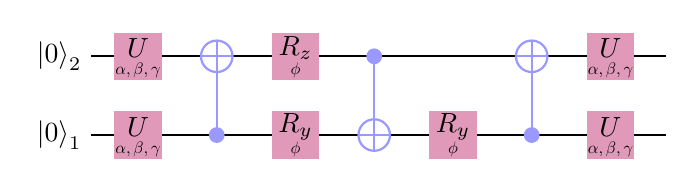
\begin{tikzpicture}[%
		measure/.pic={
			\draw[fill=black] (-3mm,-3mm) rectangle (3mm,3mm) ;
			\draw[color=white,thick] (0,-1mm) -- ([yshift=-1mm] 60:3mm)
			 (2mm,-1mm) arc [start angle=0, end angle=180, radius=2mm];
		},
		CX/.pic={
			\draw[color=blue!40,thick] (0,0) circle [radius=0.2];
			\draw[color=blue!40,thick] (-0.2,0) -- (0.2,0)  (0,-0.2) -- (0,0.2);
		}
		]
	\foreach \q/\i in {q1/1,q2/2}
	{
		\node[minimum size=6mm] (\q) at (0,\i) {$\ket{0}_\i$};
		\draw[thick] (\q) -- (7.7,\i) ;
	}
	\foreach \x/\q in {1/1,1/2,7/1,7/2}
	{
		\path[fill=blue!30!red!40] ($ (\x,\q) - (0.3,0.3) $) rectangle +(0.6,0.6);
		\node at ($ (\x,\q) + (0,.1) $) {$U$};
		\node at ($ (\x,\q) + (0,-.18) $) {\scalebox{0.6}{$\alpha,\beta,\gamma$}};
	}
	\foreach \x/\q/\a in {3/1/y,3/2/z,5/1/y}
	{
		\path[fill=blue!30!red!40] ($ (\x,\q) - (0.3,0.3) $) rectangle +(0.6,0.6);
		\node at ($ (\x,\q) + (0,.1) $) {$R_\a$};
		\node at ($ (\x,\q) + (0,-.18) $) {\scalebox{0.6}{$\phi$}};
	}
	\foreach \x/\q/\p in {2/1/2,4/2/1,6/1/2}
	{
		% CX gates
		\draw[thick,color=blue!40] (\x,\q) -- (\x,\p);
		\path[fill=blue!40] (\x,\q) circle[radius=0.1];
		\draw (\x,\p) pic {CX};
	}
\end{tikzpicture}
\end{document}
